%%%%%%%%%%%%%%%%%%%%%%%%%%%%%%%%%%%%%%%%%
% Large Colored Title Article
% LaTeX Template
% Version 1.1 (25/11/12)
%
% This template has been downloaded from:
% http://www.LaTeXTemplates.com
%
% Original author:
% Frits Wenneker (http://www.howtotex.com)
%
% License:
% CC BY-NC-SA 3.0 (http://creativecommons.org/licenses/by-nc-sa/3.0/)
%
%%%%%%%%%%%%%%%%%%%%%%%%%%%%%%%%%%%%%%%%%

%----------------------------------------------------------------------------------------
%	PACKAGES AND OTHER DOCUMENT CONFIGURATIONS
%----------------------------------------------------------------------------------------

\documentclass[DIV=calc, paper=letter, fontsize=12pt, twocolumn]{scrartcl}	 % A4 paper and 11pt font size

\usepackage{lipsum} % Used for inserting dummy 'Lorem ipsum' text into the template
\usepackage[english]{babel} % English language/hyphenation
\usepackage[protrusion=true,expansion=true]{microtype} % Better typography
\usepackage{amsmath,amsfonts,amsthm} % Math packages
\usepackage[svgnames]{xcolor} % Enabling colors by their 'svgnames'
\usepackage[hang, small,labelfont=bf,up,textfont=it,up]{caption} % Custom captions under/above floats in tables or figures
\usepackage{booktabs} % Horizontal rules in tables
\usepackage{fix-cm}	 % Custom font sizes - used for the initial letter in the document
\usepackage{titlesec}
\usepackage{graphicx}

\usepackage{sectsty} % Enables custom section titles
\allsectionsfont{\usefont{OT1}{phv}{b}{n}} % Change the font of all section commands

\usepackage{fancyhdr} % Needed to define custom headers/footers
\pagestyle{fancy} % Enables the custom headers/footers
\usepackage{lastpage} % Used to determine the number of pages in the document (for "Page X of Total")

% Headers - all currently empty
\lhead{}
\chead{}
\rhead{}

% Footers
\lfoot{}
\cfoot{}
\rfoot{ \usefont{OT1}{phv}{m}{n} \footnotesize Page \thepage\ of \pageref{LastPage}} % "Page 1 of 2"

\renewcommand{\headrulewidth}{0.0pt} % No header rule
\renewcommand{\footrulewidth}{0.0pt} % Thin footer rule

\definecolor{goldfishOrange}{RGB}{243,134,48}
\definecolor{goldfishWater}{RGB}{105,210,231}
\definecolor{goldfishClean}{RGB}{167,219,216}
\definecolor{dark-gray}{RGB}{22,22,22}

\definecolor{light-gray}{gray}{0.95}

\usepackage{lettrine} % Package to accentuate the first letter of the text
\newcommand{\initial}[1]{ % Defines the command and style for the first letter
\lettrine[lines=3,lhang=0.3,nindent=0em]{
\color{goldfishWater}
{\textsf{#1}}}{}}

\setlength{\columnsep}{2.0em}

%\titleformat{\section}
%{\color{red}\normalfont\Large\bfseries}
%{\color{red}\thesection}{1em}{}

%----------------------------------------------------------------------------------------
%	TITLE SECTION
%----------------------------------------------------------------------------------------

\usepackage{titling} % Allows custom title configuration

\newcommand{\HorRule}{\color{light-gray} \rule{\linewidth}{1pt}} % Defines the gold horizontal rule around the title

\pretitle{\vspace{-30pt} \begin{flushleft} \HorRule \fontsize{50}{50} \usefont{OT1}{phv}{b}{n} \color{goldfishWater} \selectfont} % Horizontal rule before the title

\title{{\color{goldfishOrange}Rackspace:}\\The Open Cloud Company} % Your article title

\posttitle{\par\end{flushleft}\vskip 0.5em} % Whitespace under the title

\preauthor{\begin{flushleft}\large \lineskip 0.5em \usefont{OT1}{phv}{b}{sl} \color{goldfishOrange}} % Author font configuration

\author{Nathan Jordan } % Your name

\postauthor{\footnotesize \usefont{OT1}{phv}{m}{sl} \color{dark-gray} % Configuration for the institution name
University of Nevada, Reno Department of Computer Science % Your institution

\par\end{flushleft}\HorRule} % Horizontal rule after the title

\date{} % Add a date here if you would like one to appear underneath the title block

%----------------------------------------------------------------------------------------

\begin{document}

\maketitle % Print the title

\thispagestyle{fancy} % Enabling the custom headers/footers for the first page 

%----------------------------------------------------------------------------------------
%	ABSTRACT
%----------------------------------------------------------------------------------------

\usefont{OT1}{phv}{m}{n}

\color{dark-gray}

% The first character should be within \initial{}
%\initial{H}\textbf{ere is some sample text to show the initial in the introductory paragraph of this template article. The color and lineheight of the initial can be modified in the preamble of this document.}

%----------------------------------------------------------------------------------------
%	ARTICLE CONTENTS
%----------------------------------------------------------------------------------------

\section*{\color{goldfishOrange}Introduction}

Founded in 1996 as a local ISP in a San Antonio garage, Rackspace has risen
from its humble roots to a billion dollar company. Rackspace now has offices
in Australia, the UK, the United Kingdom, Switzerland, The Netherlands, and Hong
Kong. Additionally, they also operate data centers in Texas, Illinois, Virginia, The UK,
Hong Kong and Australia. 

\section*{\color{goldfishOrange}Services}

As a large IT hosting provider targeting enterprise, Rackspace has many
services available to clients. In terms of cloud computing, Rackspace
offers everything from IaaS (Infrastructure as a Service), PaaS (Platform as a Service)
to SaaS (Software as a Service). Any kind of service offered can be integrated
with existing services, dependant on the needs of the organization.

\subsection*{\color{goldfishWater}Cloud Servers}

Cloud Servers are the crux of Rackspace's open cloud involvement. These servers are
OpenStack virtual machines running on a cluster in a Rackspace data center.
They can be spun-up or spun-down dynamically via the rackspace website, or via
the API (which will be covered later). There are nine flavors of Linux to choose
from, including free distributions like Ubuntu and CentOS and commercial distributions
like Red Hat, as well as multiple variants of Windows Server 2008 and 2012. Each
individual virtual server can have a varying level of computational resources 
allocated to it. CPU resources extend from four to eight virtual cores dependent
on the particular performance flavor you choose. RAM capacity ranges from 512MB
to 30GB and storage capacity of the instance varies from 20GB to 1.2TB.

A screenshot of the web-based cloud management tool is shown below in 
figure \ref{fig:cloudinterface}.

\begin{figure}[ht!]
\centering
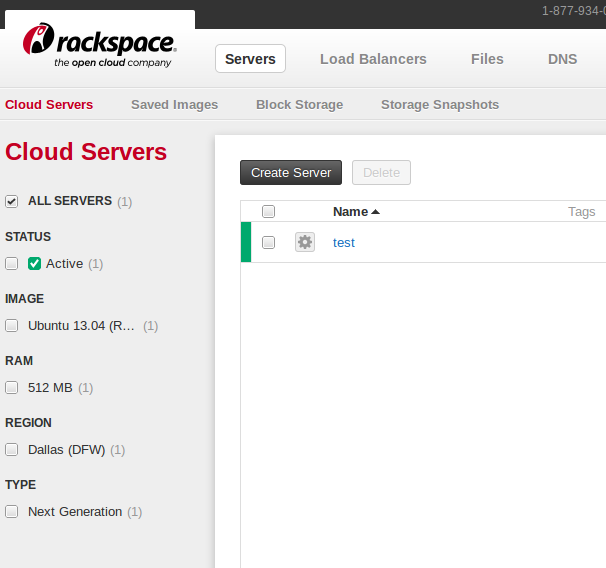
\includegraphics[width=\columnwidth]{cloudinterface.png}
\caption{Rackspace web-based cloud server management tool.}
\label{fig:cloudinterface}
\end{figure}

\subsection*{Cloud Sites}

Cloud sites offers a less technical and more problem specific solution for customers.
For customers that simply want to host a website that scales well based on
traffic demands, they might need nothing more than this. Cloud Sites offers
support for PHP and .NET environments, as well as Joomla, Drupal, DotNetNuke,
and MySQL. For clients that only require a scalable Wordpress site, the service
offers a one-click setup for creating a ready-to-go Wordpress environment. As 
mentioned previously, the service uses Rackspace cloud instances to handle 
connections, and will spawn and destroy instances when either the load becomes
too large or too small respectively. They also offer an uptime guarantee of 
99.9\%.

\subsection*{Managed Dedicated Servers}

Rackspace still offers dedicated servers to those who are not ready or comfortable
to move to a virtualized cloud environment or have special performance or security
concerns. A dedicated server, unlike their ''cloud' counterparts, is not virtualized,
and runs on bare metal. Some companies may wish to keep some services on dedicated
hardware to provide a more stable environment for the applications that they
are running or for development purposes.

Regardless of the reason, Rackspace will manage the server and ensure that it is 
running smoothly. They monitor the server for potential problems, apply security
patches as they become available, create backups, and are available for 24/7
support year-round.

\subsection*{Private Cloud}

A private cloud is a cloud that is running on an infrastructure that is dedicated
exclusively to a particular organization. It offers the flexibility of an
open cloud, with the added security usually exhibited by dedicated in-house
solutions. Rackspace can help you host your own private cloud in your own datacenter,
a datacenter of your choosing, or at a Rackspace datacenter with exclusive hardware.
Typically a private cloud is used when the organization wants to have dynamic
cloud features like dynamic instancing, but are prevented from hosting an open
cloud because of highly sensitive information being stored on the cloud or
because of organizational policy. It may also be the case that the cloud has
a very high computational demand and cannot afford to waste CPU cycles on
other clouds running on the same hardware.

\subsection*{Managed Virtualization}

In enterprise environments, virtualization is often a key piece of the IT
infrastructure. The leader of enterprise virtualization technology is 
VMWare, who's market share is greater than 80\% \cite{ref:vmware}. Rackspace
provides a managed virtualization service that allows an organization to
maintain a virtualized environment on the Rackspace cloud. The environment 
provides access to many VMWare products, including vSphere, which is a
cloud operating system. As with other managed solutions at Rackspace, 
the environment can be monitored, managed, and designed by Rackspace 
exployees who are experts in the field.

\subsection*{Cloud Files}

On the internet today, the amount of information being stored is growing
at an exponential rate. Users wanting to get access to this data will
want to be able to do so quickly and reliably. Keeping files on a single
server at one location is no longer enough. Cloud Files, much like the
name implies, allows businesses to store files in the cloud. The files
can be replicated on multiple data centers in different geographical
locations to reduce latency for users located in regions further away.
You also have access to a larger bandwidth than you would hosting
the file on your own servers. The content is delivered via the long-standing
Akamai CDN, which has been delivering content reliably since 1998.

\subsection*{Cloud Block Storage}

Cloud Files operates at the file-level, which is good for storage of
individual files that are accessed by users via the web, or by an
application using the API (such as the photos in Instagram). If you need to
mount a partition to run an operating system and your applications, 
or you want to create a drive to store files in, Rackspace has a block-level
storage service for thus purpose. Rackspace's file servers implement RAID
10 to provide a performance boost in addition to being fault tolerant.
Block storage can be allocated on traditional hard drives or solid state
drives (SSD) for dramatic performance increases in disk I/O intensive
applications.

\subsection*{Cloud Databases}

In many enterprise applications, the size of a relational database can
become exceedingly large. As the database grows, its performance will 
decrease and you may end up spending an equally large ammount on upgrading
hardware to achieve the performance that you need. By distributing the
database across multiple machines using sharding, Rackspace can scale
a MySQL database as it grows so you don't need to continue spending 
money on trying to keep up with an expanding database. Cloud databases
are stored redundantly so even in the event of a hardware failure 
your data still remains intact. Additionally, Rackspace API's can aid
you in managing your databases, including patches, configurations, 
and deployments.

\subsection*{Managed Storage}

Sometimes all you might need is a large-scale storage solution in the 
cloud. Rackspace offers all types of storage solutions to users, 
including DAS, NAS, and SAN. Performance and capabilities vary
based on the type of solution selected. Solid state disks, file-level
access, block-level access, fibre channels, replication, snapshots,
and storage-tiering are available based on which solution is chosen.
The storage is managed by Rackspace, so it can be backed up, monitored
and upgraded by storage experts.

\subsection*{Cloud Monitoring}

An important aspect of any IT solution is the ability to know when
something has gone wrong right away and resolve the issue. The Cloud
Monitoring service provided by Rackspace allows you to notify anyone
of a problem or potential problem via email or SMS. You can configure
alerts to happen individually, or send a report aggregating multiple
alerts. There are multiple types of checks that the monitoring service
can perform, including HTTP checks, PING tests, and content subjective
tests that monitor the response of your application.

\subsection*{Load Balancing}

In order to scale with the massive ammount of traffic and processing
required by large-scale applications, the workload must be distributed
across multiple machines to maintain acceptable performance. Rackspace
provides load balancers that help perform this task. Load balancers
take the incoming traffic and distribute amongst a list of nodes that
will handle the requests indipendently of eachother. The algorithm
used to distribute traffic can be changed to fit the users needs, and
includes round robin, weighted round robin, least connections, weighted
least connections, and random.

\subsection*{'RackConnect'}

Sometimes a company may want to maintain a traditional dedicated server
while still having access to the features of a dynamic cloud. This is
called a hybrid cloud and it is becoming increasingly common in enterprise
scenarios. By using a hybrid cloud, an organization can maintain their
existing dedicated infastructure and still take advantage of dynamic
cloud features, including cloud servers, cloud storage, and databases,
even when the dedicated servers are in-house at the organization.
Any cloud-based feature available to Rackspace customers can be used
by an organization without having to migrate their systems. RackConnect 
works by creating a VPN between the organization's network and Rackspace.
Security policies restrict what/who has access to the cloud features
and protects the existing company network from being compromised.

\subsection*{API Access}

All the services provided by Rackspace, would be far less effective if 
they didn't have a way for them to be managed programatically. All 
non-dedicated cloud services have API calls through various methods
(typically JSON or XML) that allow you to control every aspect of 
your cloud. This is where the real power of the Rackspace cloud
comes from. You can spin up instances and destroy them as neccessary,
create new load balancers on the fly, add files to the Akamai CDN, 
backup your data, or setup new alerts, all via the API.

\section*{Rackspace \& Amazon Web Services}

When we discuss cloud computing,

\cite{lolz}

\section*{Conclusion}

This is what I talked about.


%----------------------------------------------------------------------------------------
%	REFERENCE LIST
%----------------------------------------------------------------------------------------

\bibliographystyle{IEEEtran}
\bibliography{refs}

%\begin{thebibliography}{99} % Bibliography - this is intentionally simple in this template

%\bibitem[Figueredo and Wolf, 2009]{Figueredo:2009dg}
%Figueredo, A.~J. and Wolf, P. S.~A. (2009).
%\newblock Assortative pairing and life history strategy - a cross-cultural
%  study.
%\newblock {\em Human Nature}, 20:317--330.
 
%\end{thebibliography}

%----------------------------------------------------------------------------------------

\end{document}
